\begin{bx1}
  \begin{wrapfigure}{r}{0.3\linewidth}
    \centering
    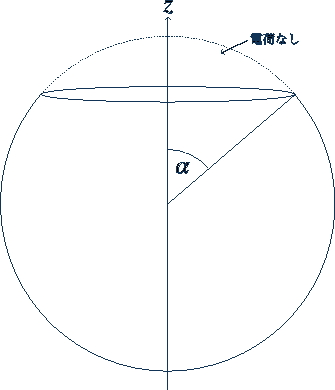
\includegraphics[width=\linewidth]{fig/Jackson3-2.pdf}%  
  \end{wrapfigure}%
  半径$R$の球が,角度$\theta =  \alpha$の円錐によって定まる北極の領域(球帽,spherical cap)
  を除いてその表面に一様な面電荷密度$Q / (4\pi R^2)$を持っている.
  \begin{enumerate}[(a)]%  
    \item  
  球の内部でのポテンシャルが次のように表されることを示せ.ただし,$l = 0$に対して
      $P_{l-1}(\cos\alpha) = -1$と約束する.
      \begin{gather}%
        \Phi = \frac{Q}{8\pi\eps_0} \sum_{l=0}^{\infty} \frac{1}{2l+1} \ab[
          P_{l+1}(\cos\alpha) - P_{l-1}(\cos\alpha)
        ] \frac{r^l}{R^{l+1}} P_l(\cos\theta).
      \end{gather}%
    また,外部領域におけるポテンシャルはどのようになるか?
  \item 
    原点における電場の大きさとその向きを決定せよ.
  \item
    北極における球帽が(1)十分に小さい極限;と(2)十分に大きく電荷が存在する部分
      が南極のごく僅かな領域のみになる;これら2つの場合について,
      (a),(b)の結果の極限について議論せよ.
  \end{enumerate}%
\end{bx1}

極角$\theta$が$\theta < \alpha$を満たす部分には電荷が存在せず,その他の部分には
一様な電荷密度$\sigma_{\mr{c}} = Q /(4\pi R^2)$が存在するような球を考える.

\itemlabel{(a)}
  ポテンシャルをLegendre多項式で展開して
  \begin{gather}%
    \Phi(r,\theta) = \sum_{l=0}^\infty \ab(A_l r^l + B_l r^{-(l+1)}) P_l(\cos\theta)
  \end{gather}%
  とする.
  球の内部で$r\to 0$としたときに発散しない条件より$l = 0, 1, \ldots$について$B_l = 0$
  また,球の外部については$r \to \infty$としたときにポテンシャルがゼロに漸近するとして,
  $l = 0, 1, \ldots$について$A_l = 0$である.
  したがって,球の内外でのポテンシャル$\Phi_{\text{in}}$および$\Phi_{\text{out}}$は
  \begin{gather}%
    \Phi_{\text{in}}(r,\theta) = \sum_{l} A_l r^l P_l(\cos\theta),\\
    \Phi_{\text{out}}(r,\theta) = \sum_{l} B_l r^{-(l+1)} P_l(\cos\theta)
  \end{gather}%
  とかける.
  ポテンシャルは$r= R$の球面上で連続であるから,
  \begin{gather}%
    \sum_l A_l R^l P_l(\cos\theta) = \sum_l B_l R^{-(l+1)}P_l(\cos\theta)
  \end{gather}%
  であり,$\ab\{P_l\}_{l=0,1,2,\ldots}$が直交関数系をなすことより
  $B_l = A_l R^{2l+1}$である.

  また,電場の接続条件は
  \begin{gather}%
    \sigma = \eps_0 \ab[\eval{\diffp{\Phi_{\text{in}}}{r}}_{r=R} -
    \eval{\diffp{\Phi_{\text{out}}}{r}}_{r=R}] 
    =
    \begin{dcases}%
      \frac{Q}{4\pi R^2} \qqtext{if} \theta \geq \alpha\\
      0 \qqtext{if} 0 \leq \theta < \alpha
    \end{dcases}%
  \end{gather}%
  である.
  \begin{gather}%
    \eval{\diffp{\Phi_{\text{in}}}{r}}_{r=R}
    - \eval{\diffp{\Phi_{\text{out}}}{r}}_{r=R} 
    = \sum_{l=0}^\infty A_l \ab(2l+1) R^{l-1} P_l(\cos\theta)
  \end{gather}%
  に注意すると,$\dl{(\cos\theta)}P_{l'}(\cos\theta)$をかけて$\cos\theta =1$から
  $\cos\theta = -1$で積分をすると,
  直交関係より以下が得られる($l,l'$の入れ替えを行った);
  \begin{gather}%
    A_l = \frac{Q}{8\pi \eps_0}\frac{1}{R^{l+1}} \int_{-1}^{\cos\alpha} \dl{x} P_l(x).
  \end{gather}%
  Legendre多項式に関する漸化式\eqref{eq:legedre_zenka1}
  より,
  \begin{gather}%
    \int_{-1}^{\cos\alpha} \dl{x} P_l(x) 
    = \frac{1}{2l+1}\ab[P_{l+1}(\cos\alpha) - P_{l-1}(\cos\alpha)]
  \end{gather}%
  である($P_{l+1}(-1) - P_{l-1}(-1) = 0$であることに注意せよ).
  したがって,
  \begin{gather}%
    A_l = \frac{Q}{8\pi \eps_0} \frac{1}{2l+1} \ab[P_{l+1}(\cos\alpha) - P_{l-1}(\cos\alpha)]\frac{1}{R^{l+1}}
  \end{gather}%
  であり,球内部のポテンシャルは
  \begin{gather}%
    \Phi_{\text{in}}(r,\theta) = \frac{Q}{8\pi \eps_0} \sum_{l=0}^\infty \frac{1}{2l+1}
    \ab[P_{l+1}(\cos\alpha) - P_{l-1}(\cos\alpha)] \frac{r^l}{R^{l+1}} P_l(\cos\theta)
  \end{gather}%
  と表される.
  また,球外部のポテンシャルについては,
  \begin{gather}%  
    \Phi_{\text{out}}(r,\theta) = \frac{Q}{8\pi \eps_0} \sum_{l=0}^\infty \frac{1}{2l+1}
    \ab[P_{l+1}(\cos\alpha) - P_{l-1}(\cos\alpha)] \frac{R^l}{r^{l+1}} P_l(\cos\theta)
  \end{gather}%
  と表される.

\itemlabel{(b)}
  電場は$\bs{E} = -\gr \Phi$で与えられるので,
  \begin{align}%  
    E_r &= -\diffp{\Phi}{r} \notag\\
    &= -\frac{Q}{8\pi \eps_0}\sum_{l=1}^\infty
    \frac{l}{2l+1}\ab[P_{l+1}(\cos\alpha) - P_{l-1}(\cos\alpha)] 
    \frac{r^{l-1}}{R^{l+1}} P_l(\cos\theta)\\
    E_\theta &= -\frac{1}{r}\diffp{\Phi}{\theta} \notag\\
    &= -\frac{1}{r}\frac{Q}{8\pi\eps_0} 
    \sum_{l=0}^\infty \frac{1}{2l+1} \ab[P_{l+1}(\cos\alpha) - P_{l-1}(\cos\alpha)]\frac{r^l}{R^{l+1}} \diff{P_l(\cos\theta)}{\theta}
  \end{align}%
  である.
  原点では$r = 0$として考えると,$E_r, E_\theta$ともに$l=1$の項だけが残るので,
  $P_2(\cos\alpha) - P_0(\cos\alpha) = -(3/2)\sin^2\al$であることなどに注意すると,
  \begin{align}%
    \bs{E}(r=0) &= \frac{Q}{16\pi\eps_0}\frac{1}{R^2}\sin^2\alpha \ab[\cos\theta \hat{\bs{r}} - \sin\theta \hat{\bs{\theta}}] \notag\\
    &= \frac{Q}{16\pi \eps_0} \frac{1}{R^2}\sin^2\al \hat{\bs{z}}
  \end{align}%
  となる.

\itemlabel{(c-1-a)}
  $\al \to 0$の極限を考える.

  $\cos\al \sim 1 - \al^2 / 2$であるから,$P_l(\cos\al) \sim P_l(1) - (\al^2/2)P_l'(1)$として
  Taylor展開できる.
  $l = 0$のときは
  \begin{gather}%
    P_1(\cos\al) - P_{-1}(\cos\al) = \cos\al + 1 \sim 2 - \frac{\al^2}{2}
  \end{gather}%
  $l \geq 1$のときは
  \begin{align}%
    P_{l+1}(\cos\al) - P_{l-1}(\cos\al) 
    &\sim -\frac{\al^2}{2}\ab(P_{l+1}'(1) - P_{l-1}'(1))\notag\\
    &= -\frac{\al^2}{2}\ab(2l+1) P_l(1) = -\frac{2l+1}{2}\al^2
  \end{align}%
  と近似されるので,
  \begin{align}%
    \Phi_{\text{in}} &\sim 
    \frac{Q}{4\pi \eps_0} \ab[\frac{1}{R} 
    - \frac{\al^2}{4}\sum_{l=0}^\infty \frac{r^l}{R^{l+1}}P_l(\cos\theta)]\notag\\
    &= \frac{Q}{4\pi\eps_0}\ab[
      \frac{1}{R} - \frac{\al^2}{4} \frac{1}{\ab|\bs{x} - R\hat{\bs{z}}|}
    ]
  \end{align}%
  とかける.
  また,球外部のポテンシャルは
  \begin{align}%
    \Phi_{\text{out}} &\sim \frac{Q}{4\pi\eps_0}\ab[
      \frac{1}{r} - \frac{\al^2}{4} \sum_{l=0}^\infty \frac{R^l}{r^{l+1}}P_l(\cos\theta)
    ]\notag\\
    &= \frac{Q}{4\pi\eps_0} \ab[
      \frac{1}{r} - \frac{\al^2}{4} \frac{1}{\ab|\bs{x} - R\hat{\bs{z}}|}
    ]
  \end{align}%
  であるから,球内外のポテンシャルは
  \begin{gather}%
    \Phi \sim \frac{Q}{4\pi\eps_0} \ab[\frac{1}{r_>} - \frac{\al^2}{4}\frac{1}{\ab|\bs{x} - R \hat{\bs{z}}|}]
  \end{gather}%
  と統一的に書くことができる.ただし,$r_>$は$r$と$R$のうち大きい方である.

\itemlabel{(c-1-b)}
  中心における電場の極限は$\sin\al \sim \al$に注意して
  \begin{gather}%
    \bs{E}(r = 0) \sim \frac{Q}{16\pi \eps_0}\frac{\al^2}{R^2} \hat{\bs{z}}
  \end{gather}%
  である.

\itemlabel{(c-2-a)}
  $\al \to \pi$の極限を考えるが,簡単のため$\beta \equiv \pi - \al \to 0$の極限を考える.
  \begin{gather}%
    \cos\al = \cos(\pi -\be) \sim -1 + \frac{\be^2}{2}
  \end{gather}%
  に注意すると,(c-1)と同様にして,
  \begin{gather}%
    P_{l+1}(\cos\al) - P_{l-1}(\cos\al) \sim (-1)^l \frac{2l+1}{2} \be^2
    \qqtext{for} l = 0, 1, \ldots
  \end{gather}%
  と表せる.したがって,
  \begin{align}%
    \Phi_{\text{in}} &\sim \frac{Q}{8\pi\eps_0} \be^2
    \frac{1}{2} \sum_{l=0}^\infty (-1)^l \frac{r^l}{R^{l+1}} P_l(\cos\theta)\notag\\
    &= \frac{Q}{16\pi\eps_0}\beta^2 \sum_{l=0}^\infty \frac{r^l}{R^{l+1}} P_l(-\cos\theta)\notag\\
    &= \frac{Q}{16\pi\eps_0} \beta^2 \frac{1}{\ab|\bs{x} + R \hat{\bs{z}}|}
  \end{align}%
  である.球外のポテンシャルも同様に計算することができて,
  \begin{gather}%
    \Phi_{\text{out}} \sim \frac{Q}{16\pi\eps_0} \beta^2 \frac{1}{\ab|\bs{x} + R \hat{\bs{z}}|}
  \end{gather}%
  となる(同じ結果を与える).

\itemlabel{(c-2-b)}
  原点での電場は$\sin\al =\sin\be \sim \be$に注意して,
  \begin{gather}%  
    \bs{E}(r=0) \sim \frac{Q}{16\pi\eps_0} \frac{\be^2}{R^2} \hat{\bs{z}}
  \end{gather}%
  と計算される.

  \begin{tcolorbox}[dashedbox]%  
    (c-1)での結果について,これは,半径$R$の球表面に総電荷$Q$が分布しており,極角$\al$の部分には
    それに加えて,表面電荷密度$-\sigma = -Q/(4\pi R^2)$が分布している状況と一致している.
    具体的に計算をすると,まず総電荷$Q$が一様に分布しているとき,球内部のポテンシャルは
    簡単な計算により
    \begin{gather}%
      \Phi_{\text{in}}^{(1)} = \frac{Q}{4\pi\eps_0} \frac{1}{R}
    \end{gather}%
    であることがわかる.次に,極角$\al$の範囲については,$\al$が十分に小さいとき,
    この部分に存在する電荷は
    \begin{align}%
      \int \dl{\Omega}R^2(-\sigma) &= -2\pi R^2\sigma \int_0^\al \dl{\theta} \sin\theta\notag\\
      &= -2\pi R^2\sigma \ab(1-\cos\al) \notag\\
      &\sim -2\pi R^2 \sigma \frac{\al^2}{2} = -\frac{\al^2}{4}Q
    \end{align}%
    である.$\al$が十分に小さいとして,この電荷を点電荷とみなすことにすると
    これが作るポテンシャルは
    \begin{gather}%
      \Phi_{\text{in}}^{(2)} = -\frac{Q}{4\pi\eps_0} \frac{\al^2/4}{\ab|\bs{x}-R\hat{\bs{z}}|}
    \end{gather}%
    となり,$\Phi_{\text{in}}^{(1)} + \Phi_{\text{in}}^{(2)}$が(c-1-a)の
    答えになっていることが確かめられる.$\Phi_{\text{out}}$については$\Phi^{(1)}$の$1/R$を$1/r$
    として考えれば良く,この結果も整合的である.
  \end{tcolorbox}
  (a)で考えたポテンシャルを図示すると図\ref{fig:3-2_normal}のようになる.
  \begin{figure}[htbp]%  
    \centering%  
    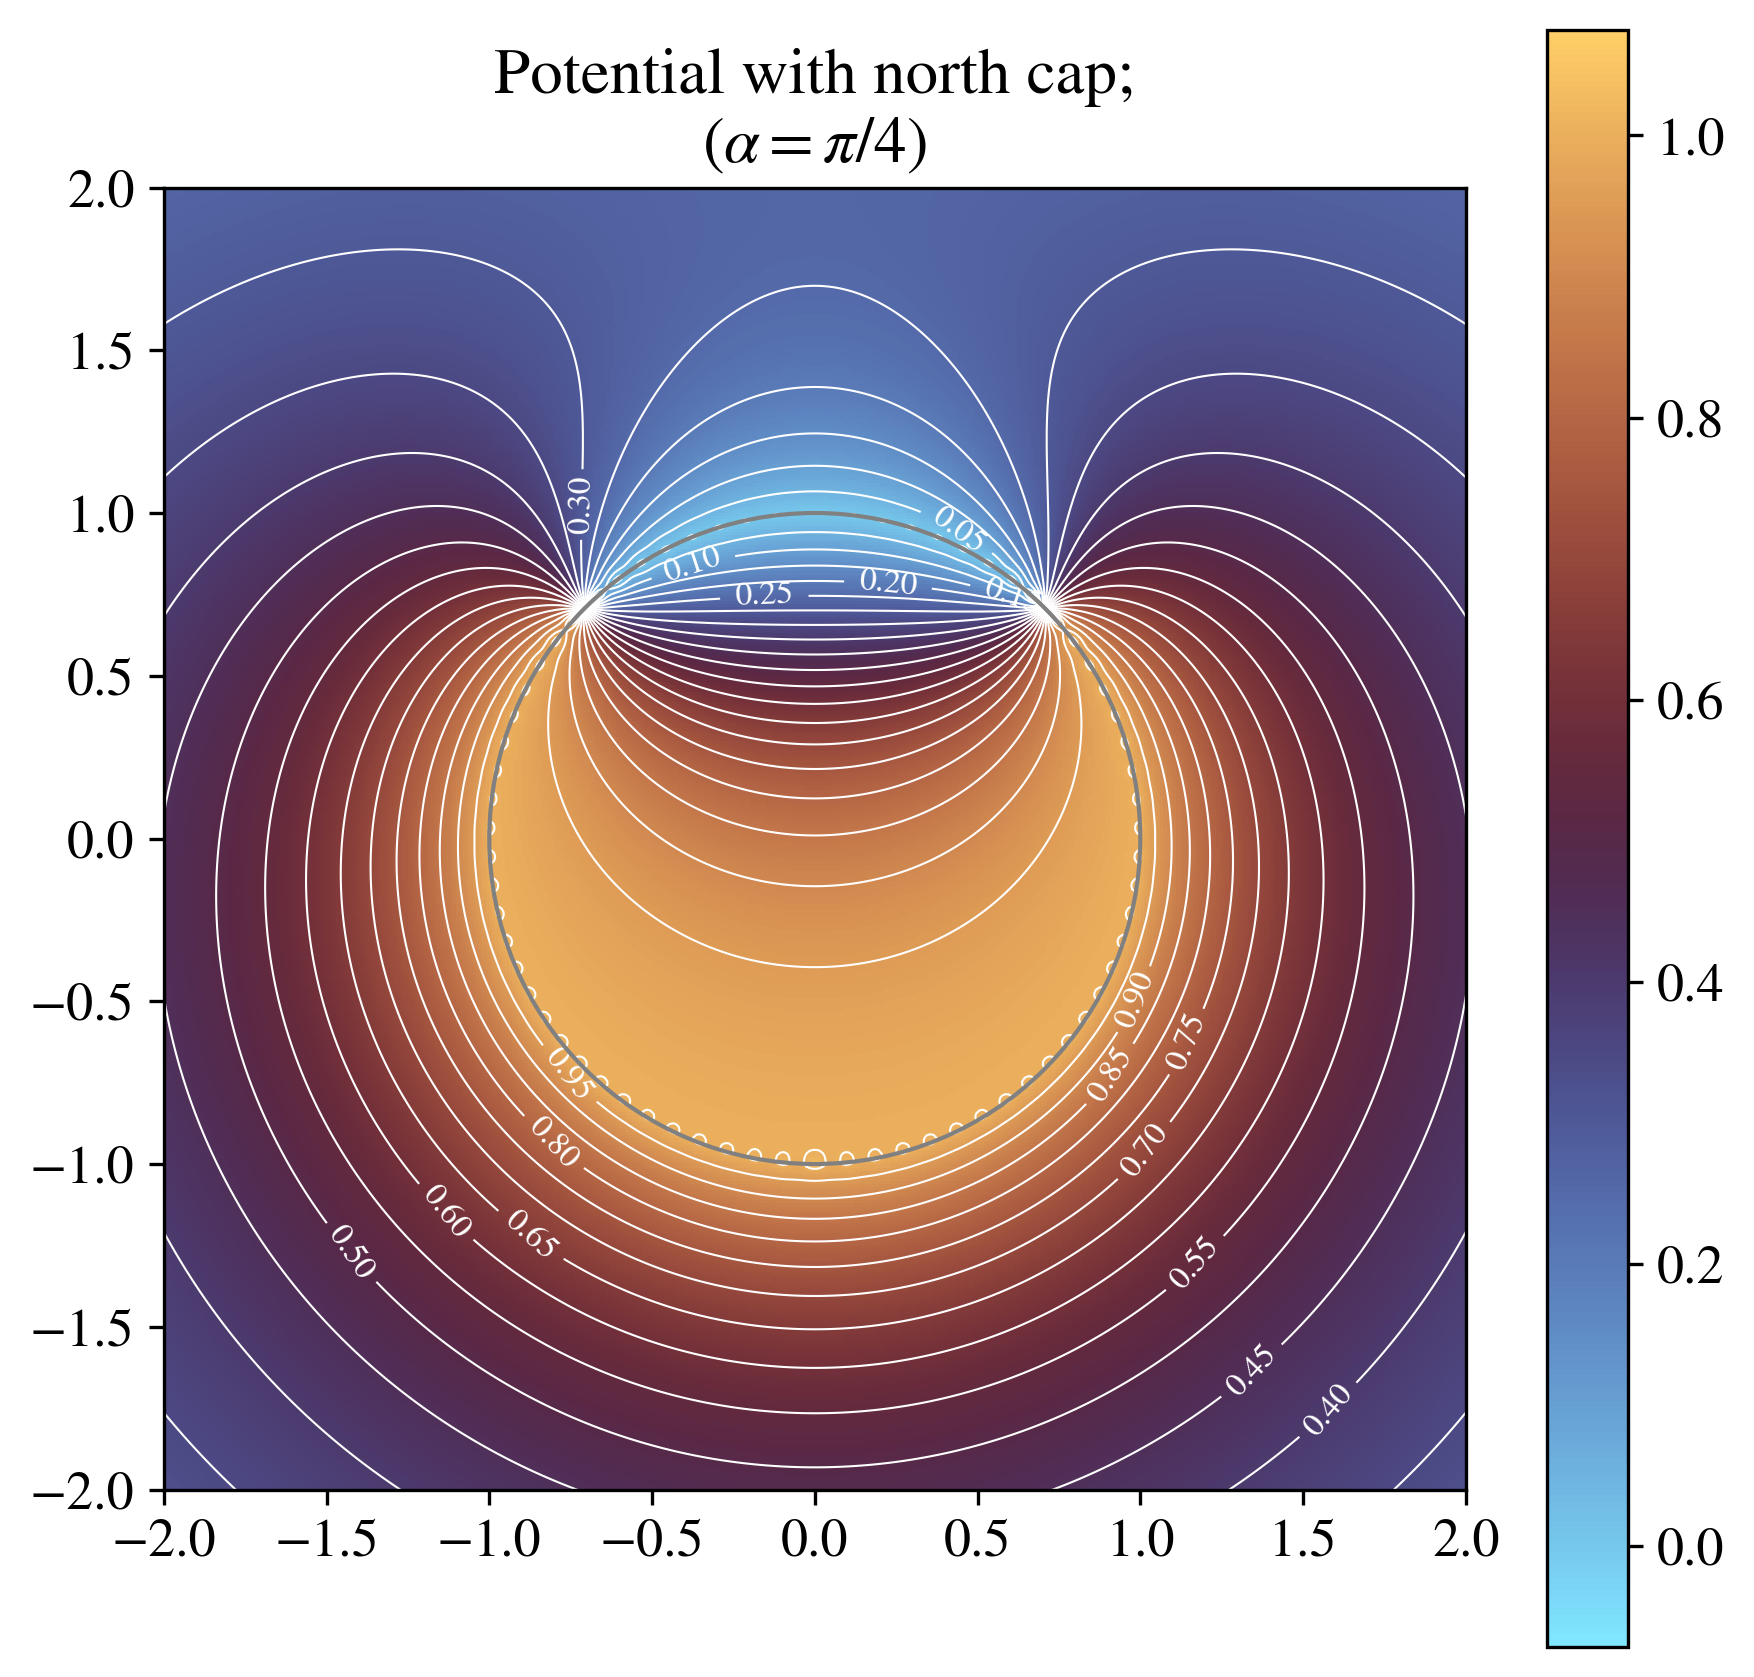
\includegraphics[width=0.5\linewidth]{py/3-2_normal.png}%  
    \caption{$\alpha = \pi/4$としてポテンシャルを描いた様子.
    ポテンシャルの単位は$Q/(4\pi\eps_0)$としており,球(図中の灰色の実線)
    の半径を$R = 1$としている.
    }%  
    \label{fig:3-2_normal}%  
  \end{figure}%

  \clearpage
